\documentclass[a4paper, 10pt]{article}

% import packages
\usepackage[margin=0.2cm]{geometry}
\usepackage{pdflscape}
\usepackage{array}
\usepackage{makecell}
\usepackage{xcolor}
\usepackage{colortbl}
\usepackage{longtable}
\usepackage{titlesec}
\usepackage{float}
\usepackage{needspace}
\usepackage{graphicx}
\usepackage{hyperref}
\usepackage{setspace}
\usepackage{fancyhdr}
\usepackage{enumitem}
\usepackage{multicol}
\usepackage{amsmath}
\usepackage{graphicx}
\usepackage[table]{xcolor}
\usepackage{booktabs}   % for \toprule, \midrule, \bottomrule
\usepackage{adjustbox}  % for \begin{adjustbox}{max width=\textwidth}
\usepackage{etoolbox}
\usepackage{tikz}
\usepackage{caption}
\usetikzlibrary{arrows.meta, positioning, shapes.geometric,fit,calc}
\usepackage{pgfplots}
\usepgfplotslibrary{groupplots}
\pgfplotsset{compat=1.18}

% ---------- custom plot styles ----------
\pgfplotsset{
  acfstyle/.style={
    ycomb,
    mark=o,
    mark size=1.0pt, % <-- smaller circles
    mark options={solid, fill=white}
  }
}


\AtBeginEnvironment{tabular}{\tiny}
\definecolor{cDark}{HTML}{203F4A}
\definecolor{cTeal}{HTML}{1D8F7E}
\definecolor{cGold}{HTML}{E9C06A}
\definecolor{cOrange}{HTML}{F29B5C}
\definecolor{cRed}{HTML}{E85D47}

\renewcommand{\familydefault}{\sfdefault}

\newlength\tindent
\setlength{\tindent}{\parindent}
\setlength{\parindent}{0pt}
\renewcommand{\indent}{\hspace*{\tindent}}

% global list spacing (affects all levels)
\setlist{noitemsep, topsep=0pt, parsep=0pt, partopsep=0pt}


% Only change level 1 itemize bullets
\setlist[itemize,1]{label=\raisebox{0.5ex}{\scalebox{0.6}{$\bullet$}}}
%\setlist[itemize,3]{label=\raisebox{0.5ex}{\scalebox{0.6}{$\bullet$}}}

% now explicitly override indentation for each level you care about:
\setlist[itemize,1]{leftmargin=1.2em}
\setlist[itemize,2]{leftmargin=1.4em}
\setlist[itemize,3]{leftmargin=0.5em}


\setlist[enumerate,1]{leftmargin=1.2em}
\setlist[enumerate,2]{leftmargin=1.4em}
\setlist[enumerate,3]{leftmargin=0.5em}

\setlength{\columnseprule}{0.1pt}
% ------------------------------------------------------


% Configure makecell package
\renewcommand{\theadalign}{bc}
\renewcommand{\theadgape}{\Gape[4pt]}
\renewcommand{\cellgape}{\Gape[4pt]}
\renewcommand{\cellalign}{lt}

% global line spacing
\renewcommand{\baselinestretch}{1.2}

% colour definitions
\definecolor{lightergray}{gray}{0.90}

\providecommand{\tightlist}{%
\setlength{\itemsep}{0pt}
\setlength{\parskip}{0pt}}

\begin{document}
  \begin{landscape}
\begin{multicols}{3}
\tiny

{\footnotesize{Analyse Prozess}}

{\scriptsize{1. Exploration \& Vorbereitung}}
\begin{itemize}
    \item Zeitreihe Input \(\rightarrow\) Technische Vorbereitung
    \item Diskrete Zeit und Kontinuierlicher Wert
    \item Erkennen der grundstruktur, erfüllung technischer Anforderungen, keine lücken, vergleichen mit erwartungen, ergänzung wenn erforderlich
\end{itemize}

{\scriptsize{2. Modellierung: Zerlegung in}}
\begin{itemize}
    \item Trend (Glatte Komponente) (deterministisch)
    \item Saisonalität (Periodische Komponente) (deterministisch)
    \item Residuen (Stoachistische Komponente) \(\rightarrow\) Stationaritätstest
    \item Getan mit libraries und oder vorwissen
\end{itemize}

{\scriptsize{3. Analyse von Residuent}}
\begin{itemize}
    \item Korrelationsanalyse
    \item Kreuzkorrelation
    \item (partielle) Autokorrelation
\end{itemize}

{\scriptsize{4. Stochastische Modellierung}}
\begin{itemize}
    \item Trend / Saisonalität \(\rightarrow\) Vorhersage Erwartung
    \item Trend / Saisonalität \(\rightarrow\) Vorhersage seltene ereignisse
    \item Korrelationsanalysen \(\rightarrow\) Stochastische Modellierung \(\rightarrow\) Extremwert analyse
    \item Korrelationen / Stochastische Modellierung \(\rightarrow\) Einsicht (Zusammenhänge)
\end{itemize}




\vspace{0.4em}
\hrule
\vspace{0.7em}

{\footnotesize{Zeitreihen statistisch charakterisieren}}

\begin{itemize}
    \item \textbf{Erwartungswert}
    \item \textbf{Varianz}
    \item \textbf{Trend}
    \begin{itemize}
        \item a long-term increasing or decreasing tendency
    \end{itemize}
    \item \textbf{Saisonalität}
    \begin{itemize}
        \item a short-term repeating pattern at fixed periods, e.g., weekly, monthly, or annually.
    \end{itemize}
    \item \textbf{Korrelationsstruktur}
    \begin{itemize}
        \item \textbf{ACF}
        \item \textbf{PACF}
        \item \textbf{CCF}
        \item \textbf{ARIMA}
        
    \end{itemize}
\end{itemize}

{\textbf{Stationarität}}

\begin{itemize}
    \item Es ändert sich nichts, voraussetzung für stochastische modellierung
    \item the concept that how a time series is changing will remain the same in the future 
    \item if statistical properties (mean, variance, and covariance) are independent of time
\end{itemize}


{\textbf{Bedingungen}} Jede separat überprüfen (wir erwarten im diagramm eine semi-gerade linie, die keinen trend zeigt
\begin{enumerate}
    \item Erwartungswert erhalten -- Ist ein Trend vorhanden?
    \begin{itemize}
        \item Augmentierter Dickey-Fuller Test (Hypothesentest H0 Prozess ist nicht stationär)
    \end{itemize}
    \item Varianz in Grenzen / unter kontrolle -- Ändert die Variabilität stark?
    \begin{itemize}
        \item 
    \end{itemize}
    \item Autokovarianz unabhängig von der Zeit -- Gibt es Regimewechsel?
\end{enumerate}

\begin{itemize}
    \item Methoden zur erreichung \(\rightarrow\) zerlegung (automatisch / manuell), differenzierung (wenn interpretierbar)
\end{itemize}

{\textbf{Zerlegung Zeitreihe \(x_n\)}}
\begin{itemize}
    \item 3 komponenten Trend \(t_n\) , Saisonalität \(s_n\), error (residuen) \(\epsilon_n\)
    \item Additive decomposition \(x_n = t_n + s_n + \epsilon_n\) (multiplicative ersetzen mit multiplikation)
\end{itemize}
    
\vspace{0.4em}
\hrule
\vspace{0.7em}


{\footnotesize{Autokorrelation}}

\begin{itemize}
    \item [1] Periodisch, [2] white noise, [3] unklar ob absteigender trend, [4] kurzlebige zusammenhänge ist nicht noise
    \item[a] steigend \(\rightarrow\) 3
    \item[b] periodisch glatt schankend \(\rightarrow\) 1
    \item[c] sinkend \(\rightarrow\) 3
    \item[d] chaotisch \(\rightarrow\) 2 keine korrelation \& 4 gibt es noch zusammenhänge?
\end{itemize}


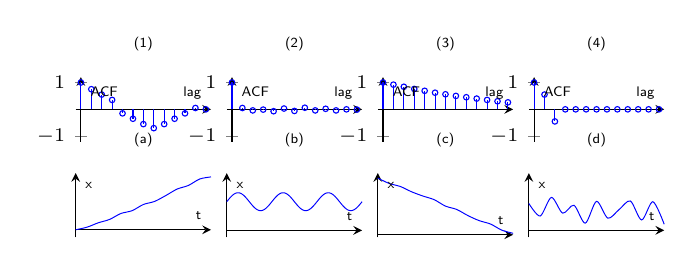
\begin{tikzpicture}
\begin{groupplot}[
  group style={
    group size=4 by 2,
    horizontal sep=0.2cm,
    vertical sep=0.4cm
  },
  width=3.3cm,
  height=2.4cm,
  axis lines=middle,
  xmin=-0.5, xmax=12.5,
  ymin=-1.2, ymax=1.2,
  xtick=\empty,
  ytick={-1,0,1},
  tick label style={font=\scriptsize},
  label style={font=\scriptsize},
  title style={font=\scriptsize},
  clip=false,
]

% ---------------- TOP ROW: ACF ----------------

% (1) alternating and dying out
\nextgroupplot[title={\tiny(1)}, xlabel={\tiny{lag}}, ylabel={\tiny{ACF}}]
\addplot+[acfstyle] coordinates {
 (0,1)
 (1,0.75) (2,0.55) (3,0.35)
 (4,-0.15) (5,-0.35) (6,-0.55) (7,-0.70)
 (8,-0.55) (9,-0.35) (10,-0.15) (11,0.05)
 (12,0)
};

% (2) only lag 0 spike
\nextgroupplot[title={\tiny(2)}, xlabel={\tiny{lag}}, ylabel={\tiny{ACF}}]
\addplot+[acfstyle] coordinates {
 (0,1)
 (1, 0.05) (2,-0.04) (3, -0.01) (4,-0.07) (5, 0.03) (6,-0.06)
 (7, 0.06) (8,-0.04) (9, 0.02) (10,-0.04) (11, 0.0) (12,-0.01)
};

% (3) positive decaying ACF
\nextgroupplot[title={\tiny(3)}, xlabel={\tiny{lag}}, ylabel={\tiny{ACF}}]
\addplot+[acfstyle] coordinates {
 (0,1)
 (1,0.92) (2,0.84) (3,0.76) (4,0.69) (5,0.62)
 (6,0.56) (7,0.50) (8,0.45) (9,0.40) (10,0.35)
 (11,0.30) (12,0.26)
};

% (4) two spikes then ~0
\nextgroupplot[title={\tiny(4)}, xlabel={\tiny{lag}}, ylabel={\tiny{ACF}}]
\addplot+[acfstyle] coordinates {
 (0,1)
 (1,0.55)
 (2,-0.45)
 (3,0) (4,0) (5,0) (6,0) (7,0)
 (8,0) (9,0) (10,0) (11,0) (12,0)
};

% ---------------- BOTTOM ROW: TIME SERIES ----------------

% (a) upward trend with small noise
\nextgroupplot[
  title={\tiny(a)},
  xmin=0, xmax=12,
  ymin=-0.3, ymax=2.2,
  xlabel={\tiny{t}}, ylabel={\tiny{x}},
  ytick=\empty
]
\addplot+[smooth, mark=none,line width=0.35pt] coordinates {
 (0,0.0) (1,0.10) (2,0.27) (3,0.40) (4,0.63) (5,0.74)
 (6,0.98) (7,1.10) (8,1.33) (9,1.58) (10,1.72) (11,1.97) (12,2.05)
};

% (b) oscillation
\nextgroupplot[
  title={\tiny(b)},
  xmin=0, xmax=12,
  ymin=-0.2, ymax=1.6,
  xlabel={\tiny{t}}, ylabel={\tiny{x}},
  ytick=\empty
]
\addplot+[smooth, mark=none,line width=0.35pt, samples=200, domain=0:12]
  {0.8 + 0.25*sin(deg(2*pi*x/4))};

% (c) downward trend with noise
\nextgroupplot[
  title={\tiny(c)},
  xmin=0, xmax=12,
  ymin=-0.1, ymax=2.2,
  xlabel={\tiny{t}}, ylabel={\tiny{x}},
  ytick=\empty
]
\addplot+[smooth, mark=none,line width=0.35pt] coordinates {
 (0,2.02) (1,1.83) (2,1.72) (3,1.53) (4,1.38) (5,1.25)
 (6,1.02) (7,0.90) (8,0.68) (9,0.50) (10,0.38) (11,0.16) (12,0.05)
};

% (d) stationary noise around constant level
\nextgroupplot[
  title={\tiny(d)},
  xmin=0, xmax=12,
  ymin=-0.2, ymax=1.6,
  xlabel={\tiny{t}}, ylabel={\tiny{x}},
  ytick=\empty
]
\addplot+[smooth, mark=none, line width=0.35pt] coordinates {
 (0,0.75) (1,0.40) (2,0.92) (3,0.48) (4,0.70) (5,0.2)
 (6,0.81) (7,0.34) (8,0.58) (9,0.82) (10,0.29) (11,0.80) (12,0.17)
};

\end{groupplot}
\end{tikzpicture}

\vspace{0.4em}
\hrule
\vspace{0.7em}

\begin{itemize}
    \item {\textbf{Regelmässige Abtastung}} einteilung kontinuierliche Daten in Punkte (diskrete Zeit)
    \item {\textbf{Lag}} Zeitspanne vom einen zeitpunkt zum nächsten
    \item {\textbf{Extrapolation}} neue Daten ausserhalb der Zeitreihe, darf nicht machen, weil würde Modell auf sich selbst anwenden
    \item {\textbf{Interpolation / Imputation}} füllen Lücken innerhalb der Daten. Lineare Interpolation: Mit dem mittelwert zwischen zwei Zeitpunkten ergänzen. Forward / Backward Fill: jetztiger Zeitpunkt und fülle alle damit bis zum nächsten (ist schlechter). Kallman-Filter: guter filter für lange lückenmit viel struktur
    \item {\textbf{LOESS}} Seasonal Trend Decompose (STL), Multi- STL (MSTL)
    \item {\textbf{Parsimonous Model}} model kommt mit weniger parameter (bevorzugen) gleich gut wie mit mehr
    \item {\textbf{Kovarianten}} Die x externe faktoren
    \item {\textbf{Scheinkorrelation}} sieht korreliert aus hat aber nichts damit zu tun
    \item {\textbf{Granger kausalität}} Leading indicator, zeigt in die zukunft für die trailing variabel
    \item {\textbf{}}
    \item {\textbf{}}
    \item {\textbf{}}
\end{itemize}

\vspace{0.4em}
\hrule
\vspace{0.7em}




\end{multicols}
\end{landscape}
\end{document}
